\chapter{Spectral Analysis}

%TODO: Introduction to fourier transform: Why is it needed/important
%TODO: Explain relation of depth in fourier transform
% -> Example: fourier transform of plane at constant depth (att. layer) is along a line in fourier space with certain slope. 
% -> Show example with simple texture + fourier transform
%TODO: Explain the spectral support of LF
%TODO: Fourier slice theorem

This chapter is intended to give an overview of the spectral properties and limitations specific to multiplicative light field displays.
Spectral analysis is a crucial method for the quality assessment and it is the origin of a comprehensive understanding of 3D displays. 
A light field emitted by the display can be interpreted as a signal that is composed of sine waves with different amplitude, phase and frequency.
Section~\ref{sec:Definitions} introduces the Fourier transform, an operation that decomposes such a signal into the frequencies that produce it.
The spectral support, i.e. the range of frequencies the display is able to produce, is analyzed in section~\ref{sec:Spectral_Support}. 

\section{Definitions}
\label{sec:Definitions}

The \textbf{Fourier transform} $\hat{f}$ of an integrable function $f \colon \mathbb{R}^n \to \mathbb{C}$ is defined as 
\begin{equation}
	\hat{f}(\xi) = \mathcal{F}(f)(\xi) \coloneqq \int_{\mathbb{R}^n} f(x) e^{-2 \pi \mathrm{i} x \cdot \xi} \, \mathrm{d}x
\end{equation}
for any $\xi \in \mathbb{R}^n$. 
According to the Fourier integral theorem, if both $f$ and $\hat{f}$ are absolutely integrable and $f$ is continuous, then the inverse transform 
\begin{equation}
	f(x) = \mathcal{F}^{-1}(\hat{f})(x) \coloneqq \int_{\mathbb{R}^n} \hat{f}(\xi) e^{2 \pi \mathrm{i} x \cdot \xi} \, \mathrm{d}\xi
\end{equation}
is well defined.
The domain of $f$ is called the \textbf{spatial domain} and the domain of $\hat{f}$ is referred to as the \textbf{frequency domain}.
An important property of the Fourier transform is that a convolution in the spatial domain becomes a multiplication in the frequency domain, or in other words, 
\begin{equation}
	\widehat{(f \ast g)}(\xi) = \hat{f}(\xi) \cdot \hat{g}(\xi)
\end{equation}
for integrable functions $f, g \colon \mathbb{R}^n \to \mathbb{C}$.
On the other hand, a multiplication in the spatial domain becomes a convolution in the frequency domain after applying the Fourier transform, that is
\begin{equation}
	\widehat{(f \cdot g)}(\xi) = (\hat{f} \ast \hat{g})(\xi).
\end{equation}

\section{The Fourier Slice Theorem}
%TODO: Explain usage of the theorem in this work

As in section~\ref{sec:light_attenuation_model}, let $p(\theta, \rho)$ be the parallel projection
The Fourier Slice Theorem, also known as the Projection-Slice Theorem, states that 


\section{Spectral Support of Light Fields}

\begin{figure}
	\subfigure[]{
		\documentclass{standalone}
\usepackage{tikz}
\usepackage{pgfplots}

\tikzset{align at bottom/.style={baseline=(current bounding box.south)}}

\begin{document} 
	\begin{tikzpicture}[scale = 0.27]
	
		\draw[->] (-5, 0) -- (5, 0) node[right] {$s$};
		\draw[<-] (-5, -5) -- (-5, 5) node[above] {$z$};
	
		\begin{scope}
			\clip (-5, -5) rectangle (5, 5);
			\draw[scale = 1, smooth, domain = -10 : 10, variable = \x, black, dashed] plot ({\x}, {3});
			\draw[scale = 1, smooth, domain = -10 : 10, variable = \x, black, dashed] plot ({\x}, {-2});
		\end{scope}
		
		\node[left] at (-5, 3) {$Z_\textrm{min}$};
		\node[left] at (-5, -2) {$Z_\textrm{max}$};
		
		\draw[very thick, blue] (0, 3) -- (2, 3);
		\draw[very thick, red] (-3, -2) -- (0, -2);
		
	\end{tikzpicture}
\end{document}
		\label{fig:two_objects}
	}
	\hfill
	\subfigure[]{
		\documentclass{standalone}
\usepackage{tikz}
\usepackage{pgfplots}

\tikzset{align at bottom/.style={baseline=(current bounding box.south)}}

\begin{document} 
	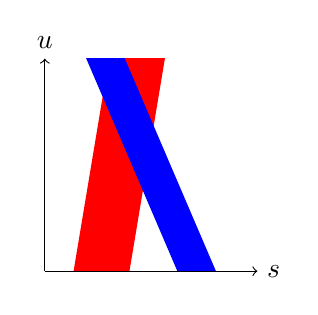
\begin{tikzpicture}[scale = 0.27]
	
		\begin{scope}
			\clip (-5, -5) rectangle (5, 5);
			\draw[scale = 1, smooth, variable = \x, red, line width = 0.7cm] plot ({\x}, { 12 / 2 * (\x + 1.5)});
			\draw[scale = 1, smooth, variable = \x, blue, line width = 0.45cm] plot ({\x}, { -7 / 3 * \x});
		\end{scope}
		
		\draw[->] (-5, -5) -- (5, -5) node[right] {$s$};
		\draw[->] (-5, -5) -- (-5, 5) node[above] {$u$};
		
	\end{tikzpicture}
\end{document}
		\label{fig:epi_two_objects}
	}
	\hfill
	\subfigure[]{
		\documentclass{standalone}
\usepackage{tikz}
\usepackage{pgfplots}

\tikzset{align at bottom/.style={baseline=(current bounding box.south)}}

\begin{document}
	\begin{tikzpicture}[scale = 0.27]
	
		\draw[->] (-5, 0) -- (5, 0);
		\draw[->] (0, -5) -- (0, 5);
		\node[right] at (5, 0) {$\xi_s$};
		\node[above] at (0, 5) {$\xi_u$};
		
		\begin{scope}
			\clip (-5, -5) rectangle (5, 5);
			\draw[scale=1, smooth, domain = -10 : 10, variable = \x, blue] plot ({\x},{ -1 / (- 7 / 3) * \x});
			\draw[scale=1, smooth, domain = -10 : 10, variable = \x, red] plot ({\x},{ -1 / (12 / 2) * \x});
		\end{scope}
		
	\end{tikzpicture}
	
\end{document}
		\label{fig:epi_fourier_transform_1}
	}
	\caption{(a) Two objects (red and blue) placed at the bounds of the depth range. 
			 (b) The EPI representing the 2D light field of the scene.
			 (c) Fourier transform of the EPI. The red and blue line mark the bounds for the spectral support.}
\end{figure}


\section{Spectral Support of Multiplicative Displays}
\label{sec:Spectral_Support}

Consider a scene with a bounded depth range $Z_{\text{min}} \leq Z \leq Z_{\text{max}}$.
In section~\ref{sec:Visualization}, it was shown that an object at a certain depth will be represented in the EPI as a line with a slope proportional to the depth.



Now, consider a single attenuation layer. 
The light field emitted by this layer has constant depth and thus, the lines in the EPI all have the same slope.


